\documentclass{report}

\usepackage{graphicx}
\usepackage[utf8]{inputenc}
\usepackage[T1]{fontenc}
\usepackage[croatian]{babel}
\usepackage{float}
\usepackage[top=3cm,bottom=3cm,left=3cm, right=4cm]{geometry}

\graphicspath{{Slike/}}

\title{Konfiguracija računala}
\author{Rikard Grandverger}
\date{January 2024}

\begin{document}

\maketitle
\tableofcontents
\listoffigures

\pagebreak

\chapter{Moćno računalo za videoigre}

\section{Svrha računala}
Svrha ovog računala je pružiti izuzetno visoku razinu performansi i grafičke snage kako bi omogućilo fluidno i visokokvalitetno iskustvo igranja video igara.

\section{Namjena računala}
Neke od namjene ovog izuzetnog računala bile bi igranje zahtjevnih videoigara, virtualna stvarnos, mogli bi snimati i uživo prijenositi sadržaj bez teškoća, ali možemo ga koristiti i za zahtjevne profesionalne programe poput AutoCAD-a, Blendera itd.

\pagebreak

\chapter{Komponente}

\section{Procesor - AMD Ryzen 9 7900X3D}
\begin{figure}[H]
    \centering
    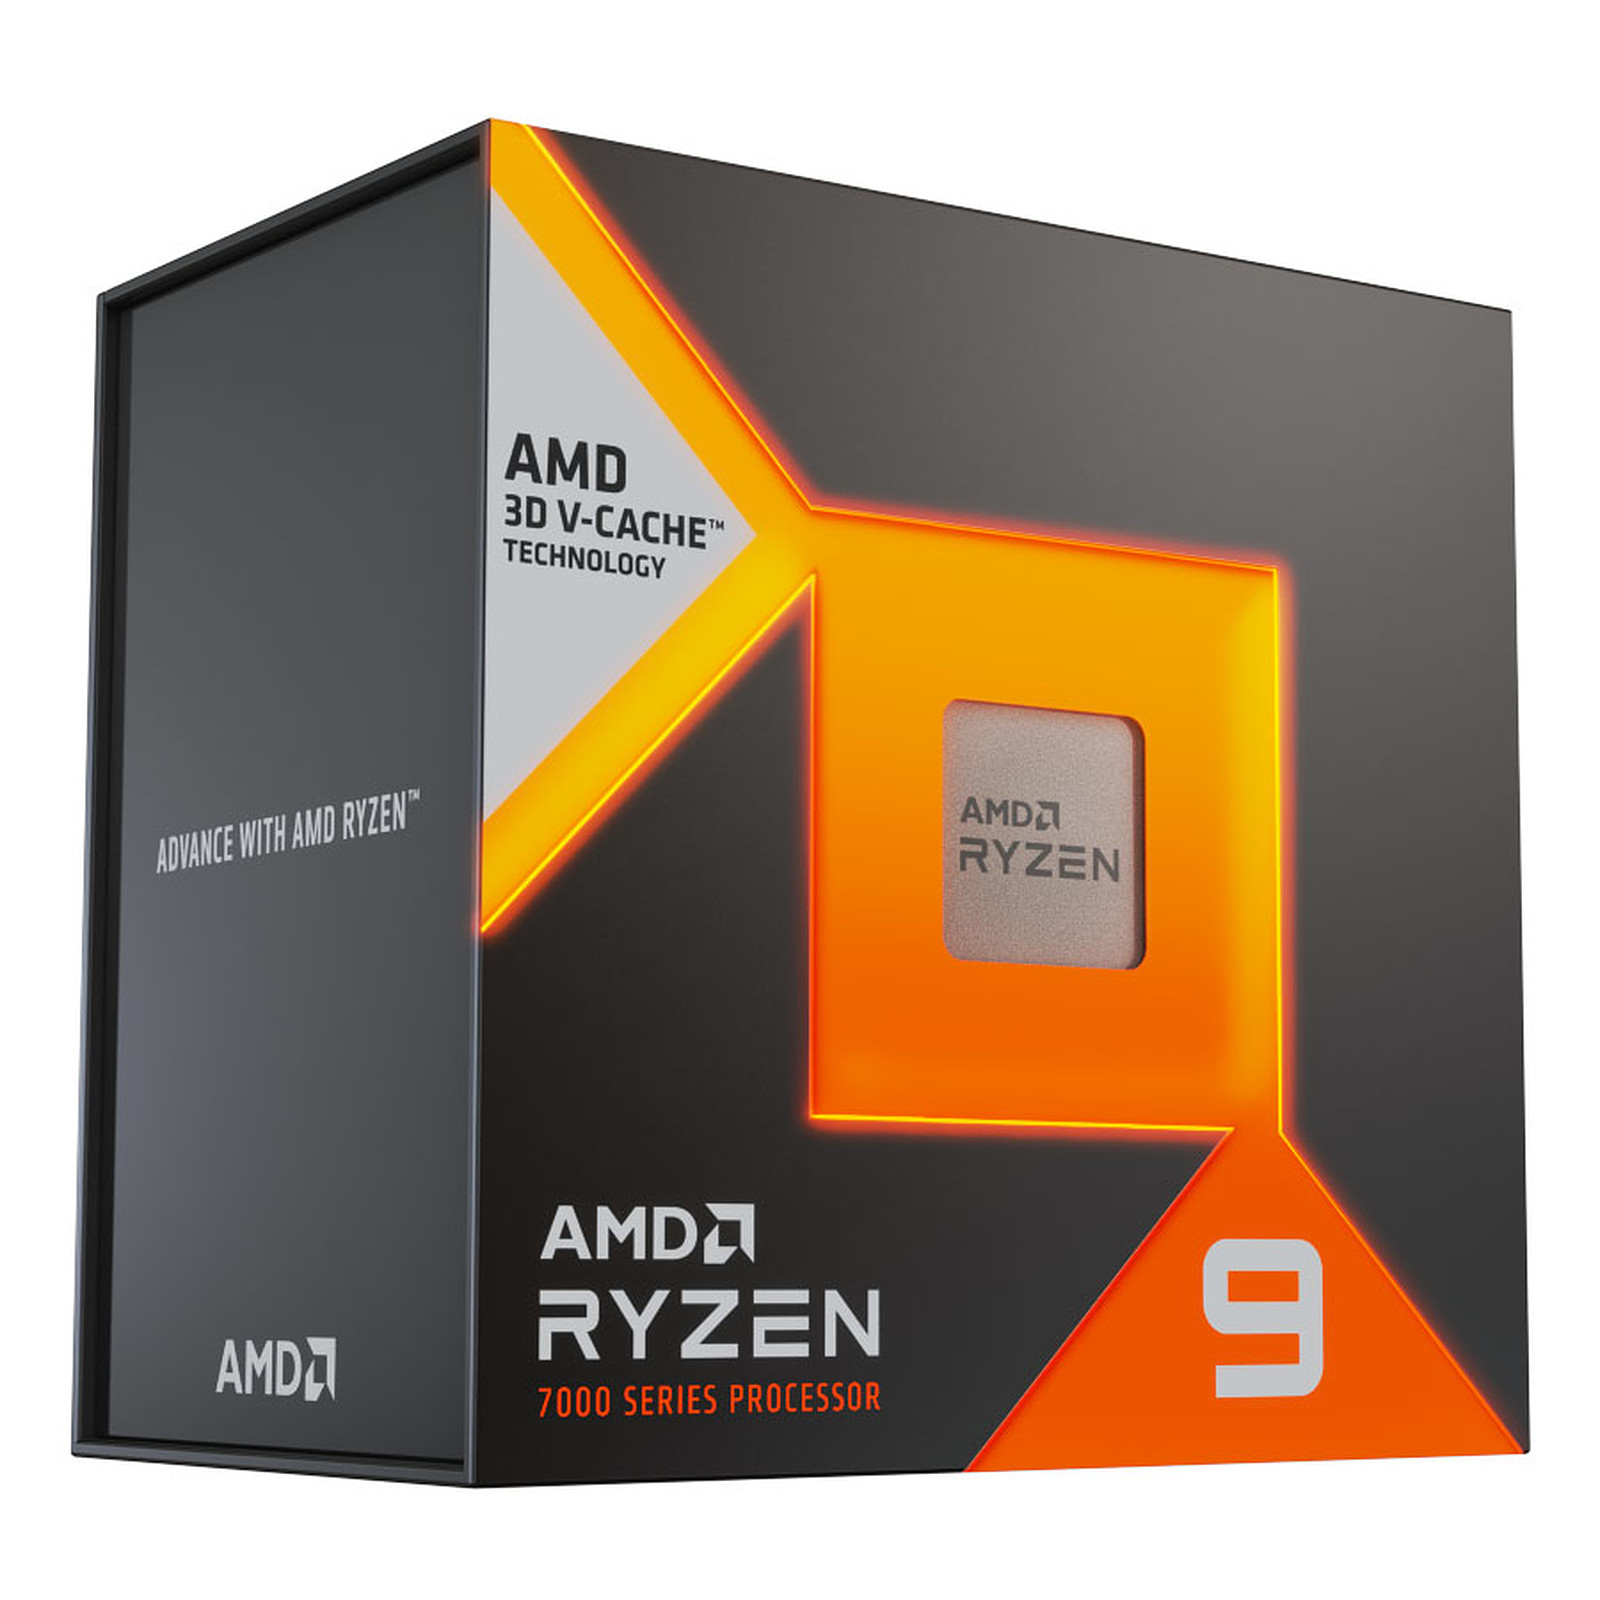
\includegraphics[scale=0.1]{Slike/7900x3d.jpg}
    \caption{AMD Ryzen 9 7900X3D}
    \label{fig:Procesor}
\end{figure}
Broj jezgara: 12\\Broj dretvi: 24\\Base clock: 4.4GHz\\Max boost clock: 5.6GHz\\L1 Cache: 768KB\\L2 Cache:12MB\\L3 Cache:    128MB\\Default TDP: 120W\\CPU Socket: AM5\\ \\Razlog: Iznimno moćan procesor koji trenutačno nema konkurencije na tržištu u vidu performansi.\\\\Cijena: 659.99 € - https://www.links.hr/hr/procesor-amd-ryzen-9-7900x3d-box-s-am5-4-4ghz-128mb-cache-12-core-bez-hladnjaka-010501030

\pagebreak

\section{Matična ploča - Asus ROG Strix X670E-E}
\begin{figure}[H]
    \centering
    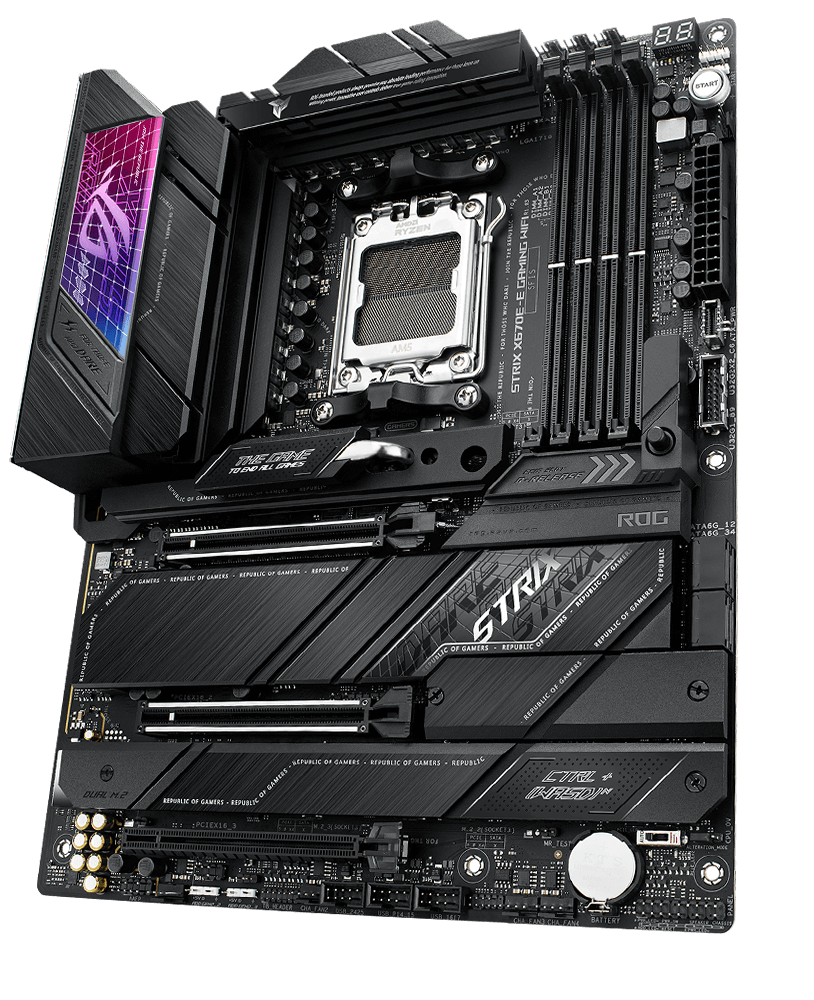
\includegraphics[scale=0.2]{Slike/ROG-Strix-X670E-E-Gaming.png}
    \caption{Asus ROG Strix X670E-E}
    \label{fig:Maticna}
\end{figure}
Chipset: AMD X670\\CPU Socket: AM5\\Slotovi za memoriju: 4x288-Pin\\Tip DDR-a: DDR5\\ Veličina: ATX\\\\Ralozg: Matična ploča koja će moći podržati sve najnovije komponente bez da ih usporava i da ima problema s povezivošću.\\\\Cijena: 601,88 € - https://www.instar-informatika.hr/maticna-ploca-asus-rog-strix-x670e-e-gaming-wifi-amd-am5-wifi-bluet/153942/product/

\pagebreak

\section{Grafička kartica - ASUS ROG Strix GeForce RTX™ 4090}
\begin{figure}[H]
    \centering
    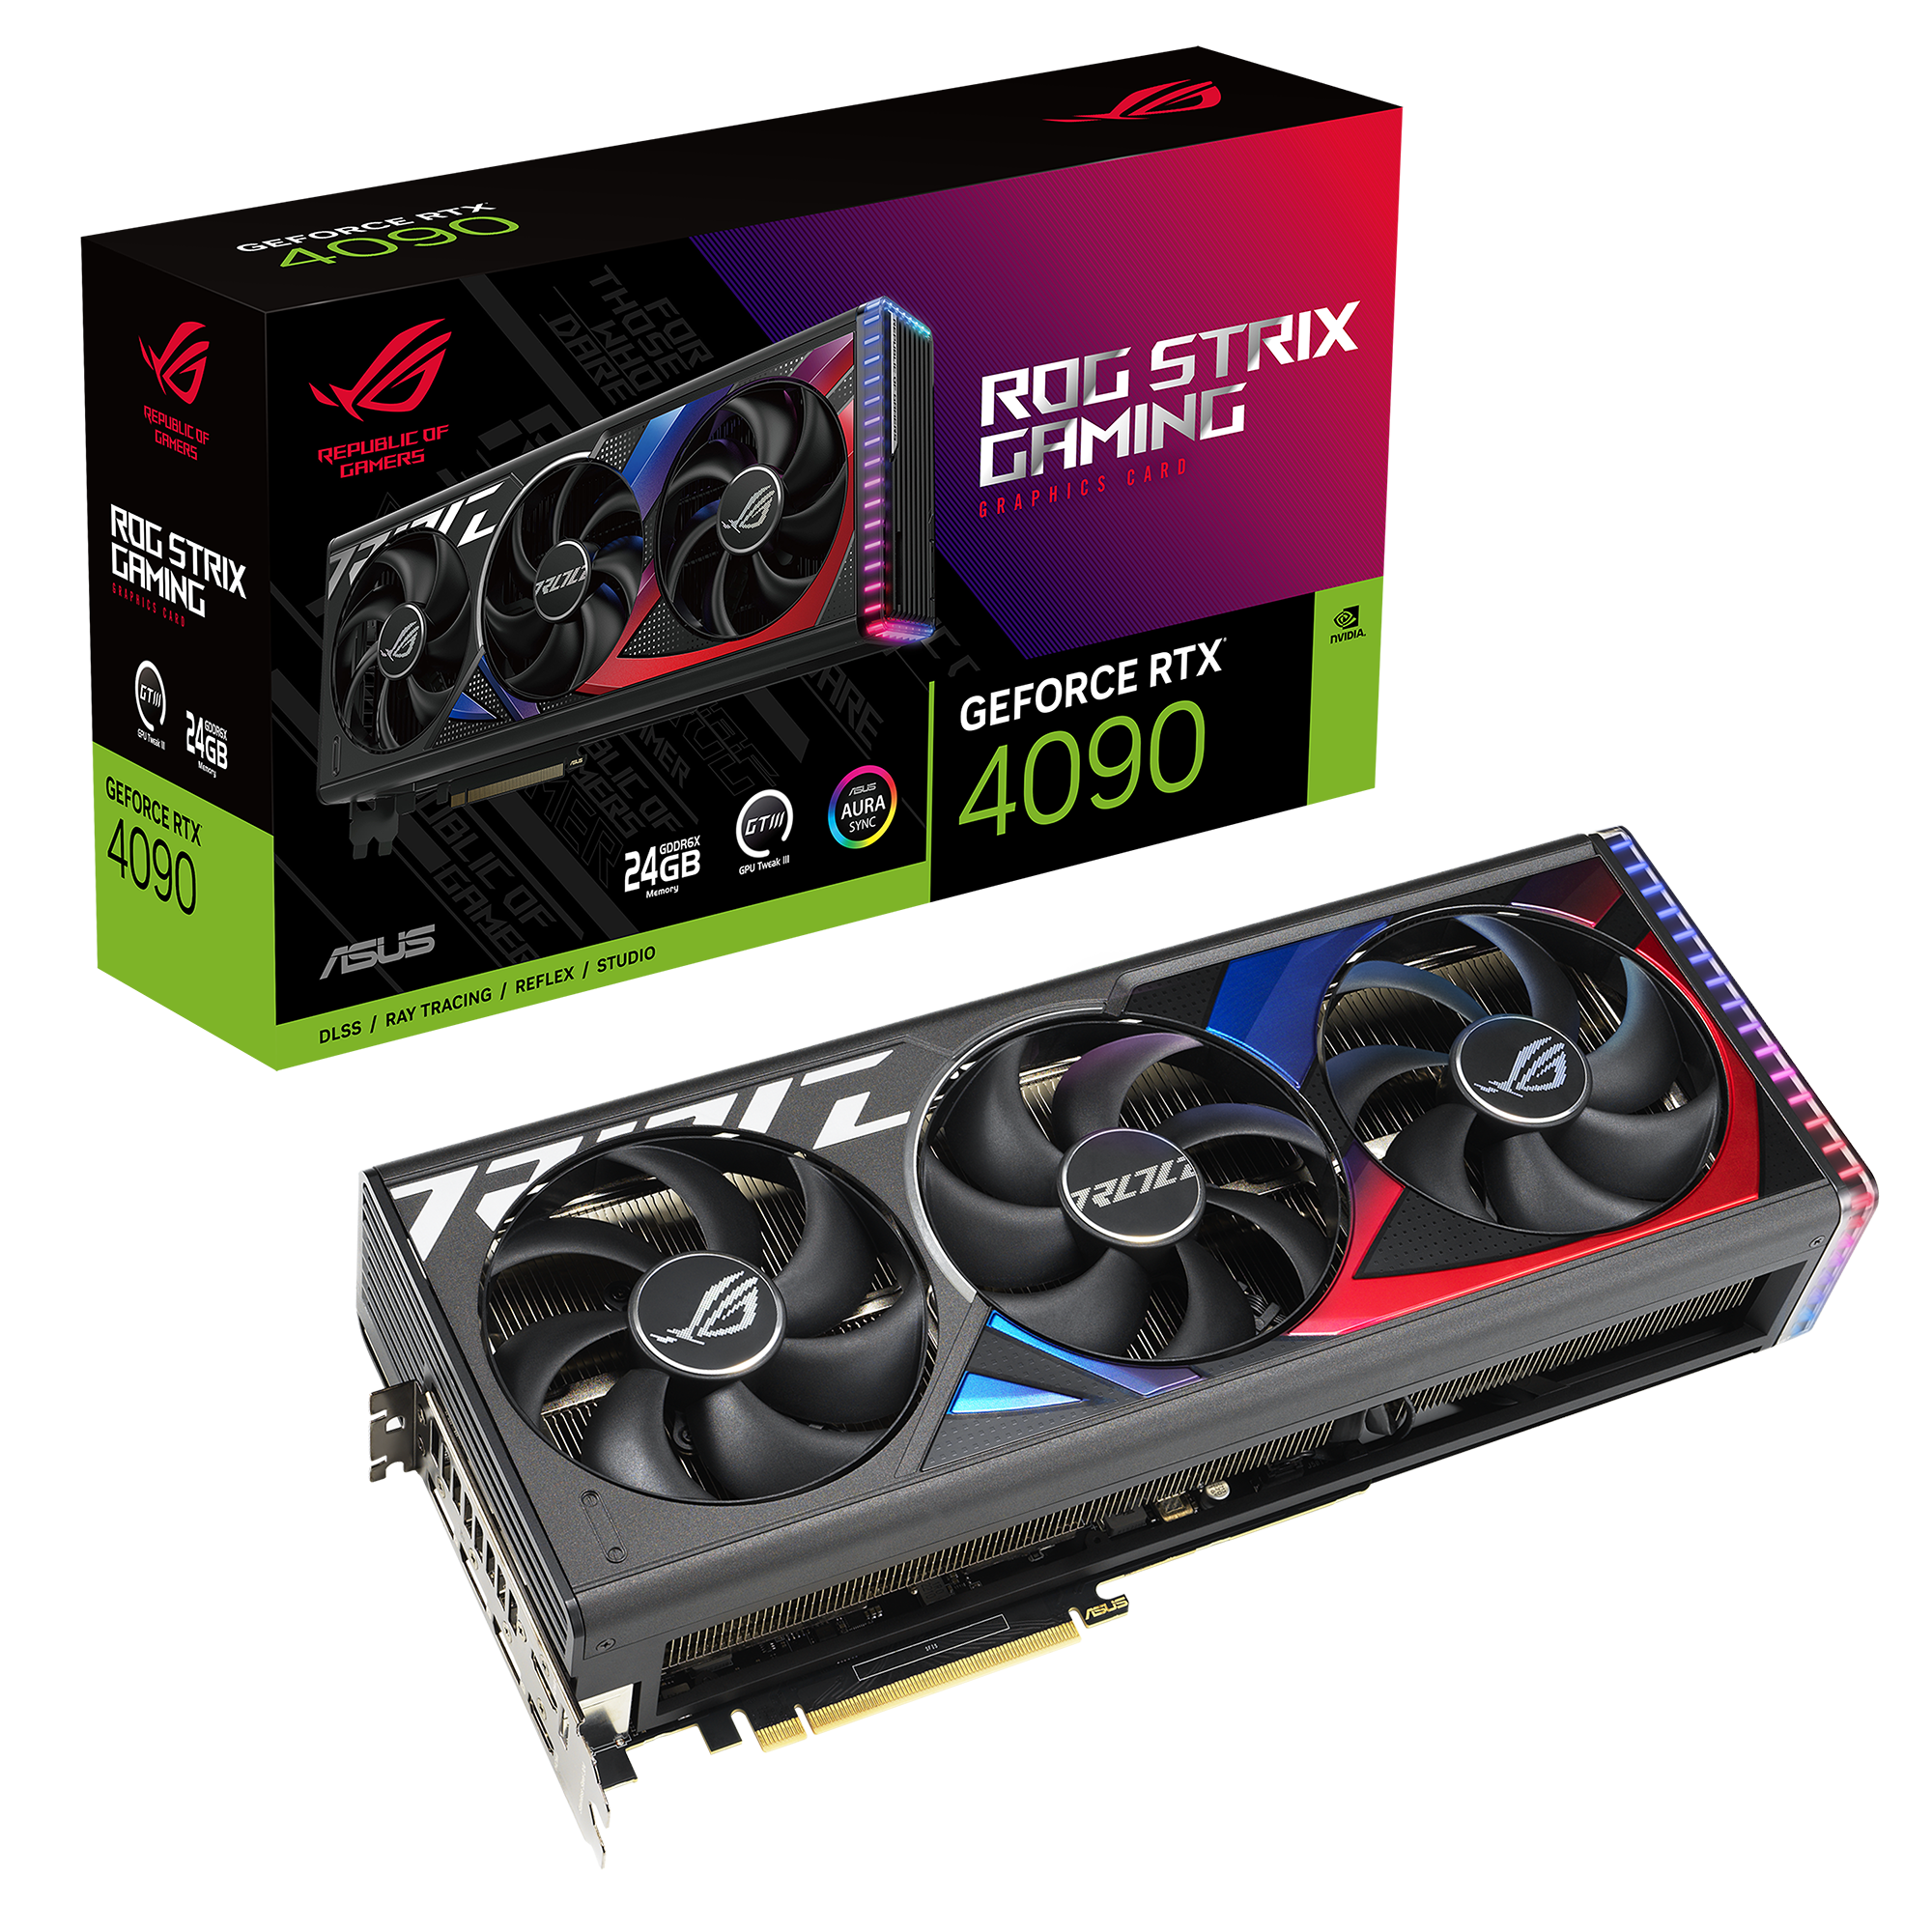
\includegraphics[scale=0.13]{Slike/rtx4090.png}
    \caption{ASUS ROG Strix GeForce RTX™ 4090}
    \label{fig:graficka}
\end{figure}
BUS: PCI Express 4.0\\OpenGL: OpenGL 4.6\\Video memorija: 24GB GDDR6X\\Brzina: 2230 MHz\\Boost brzina: 2640MHz\\CUDA jezgri: 16384\\\\Razlog: Najnovija i najjača grafička karta, trenutačno bez konkurencije na tržištu. Omogućit će nam sve što nam je potrebno.\\\\Cijena: 2.632,00 € - https://team-media.hr/proizvod/asus-rog-strix-geforce-rtx-4090-oc-grafikkarte-24gb-gddr6x-2x-hdmi-3x-dp/?utm\_source=nabava.net\&utm\_campaign=nabava.net\&utm\_medium=click

\pagebreak

\section{RAM memorija - G.Skill Trident Z5 RGB DDR5}
\begin{figure}[H]
    \centering
    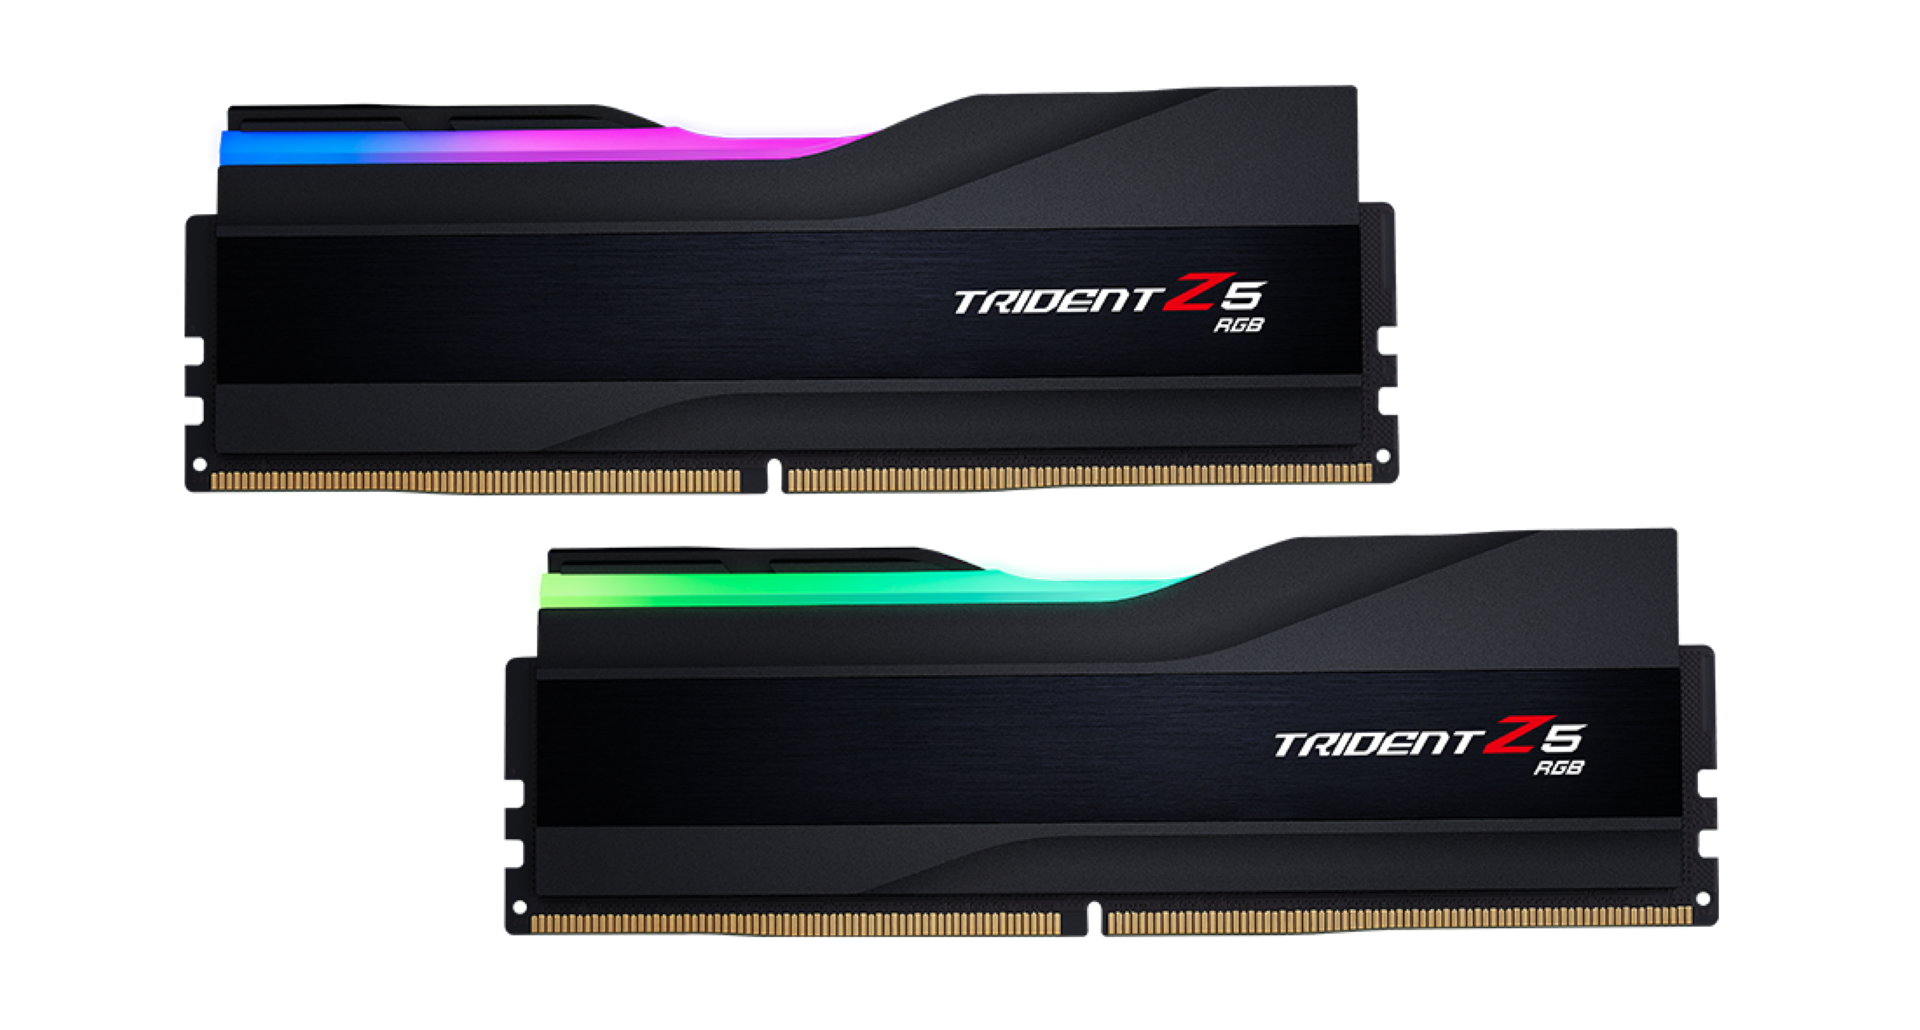
\includegraphics[scale=0.17]{Slike/gskillram.png}
    \caption{G.Skill Trident Z5 RGB DDR5 (2 x 16GB) DDR5 6400}
    \label{fig:ram}
\end{figure}
Tip memorije: DDR5\\Kapacitet: 32GB (16GBx2)\\Latencija: 32-39-39-102\\Brzina: 6400MHz\\\\Razlog: Memorija izvrsne brzine i 32GB ram-a će biti apsolutno dovoljno i za najteže zadatke.\\\\Cijena: 163,35 € - https://www.instar-informatika.hr/memorija-gskill-trident-z5-rgb-32gb-2x16gb-ddr5-6400mhz-cl32/148852/product/

\pagebreak

\section{Pohrana - Samsung 990 Pro (4TB)}
\begin{figure}[H]
    \centering
    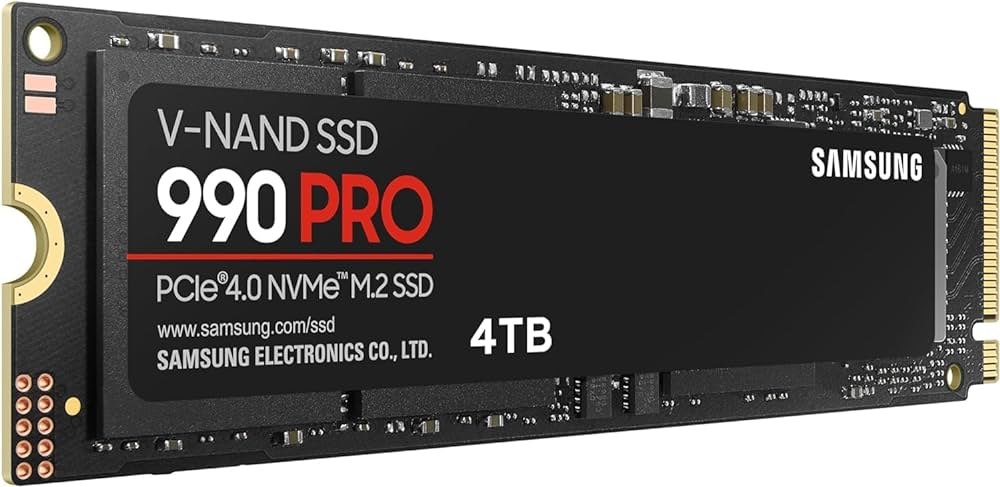
\includegraphics[scale=0.22]{Slike/ssd.jpg}
    \caption{Samsung 990 Pro}
    \label{fig:ssd}
\end{figure}
Kapacitet: 4TB\\Brzina čitanja: 7450MB/s\\Brzina pisanja: 6450MB/s\\Tip: M.2\\Temperatura: 0-70℃\\\\Razlog: Pouzdan i brz SSD s velikim kapacitetom koji će nam omogućiti pohranu svih aplikacija i videoigara.\\\\Cijena: 464,00 € - https://www.uzishop.hr/-ssd-m2-pcie-40/129836-ssd-4tb-m2-80mm-pci-e-40-x4-nvme-v-nand-samsung-990-pro-mz-v9p4t0bw.html

\pagebreak

\section{Kućište - Cooler Master HAF 700 EVO}
\begin{figure}[H]
    \centering
    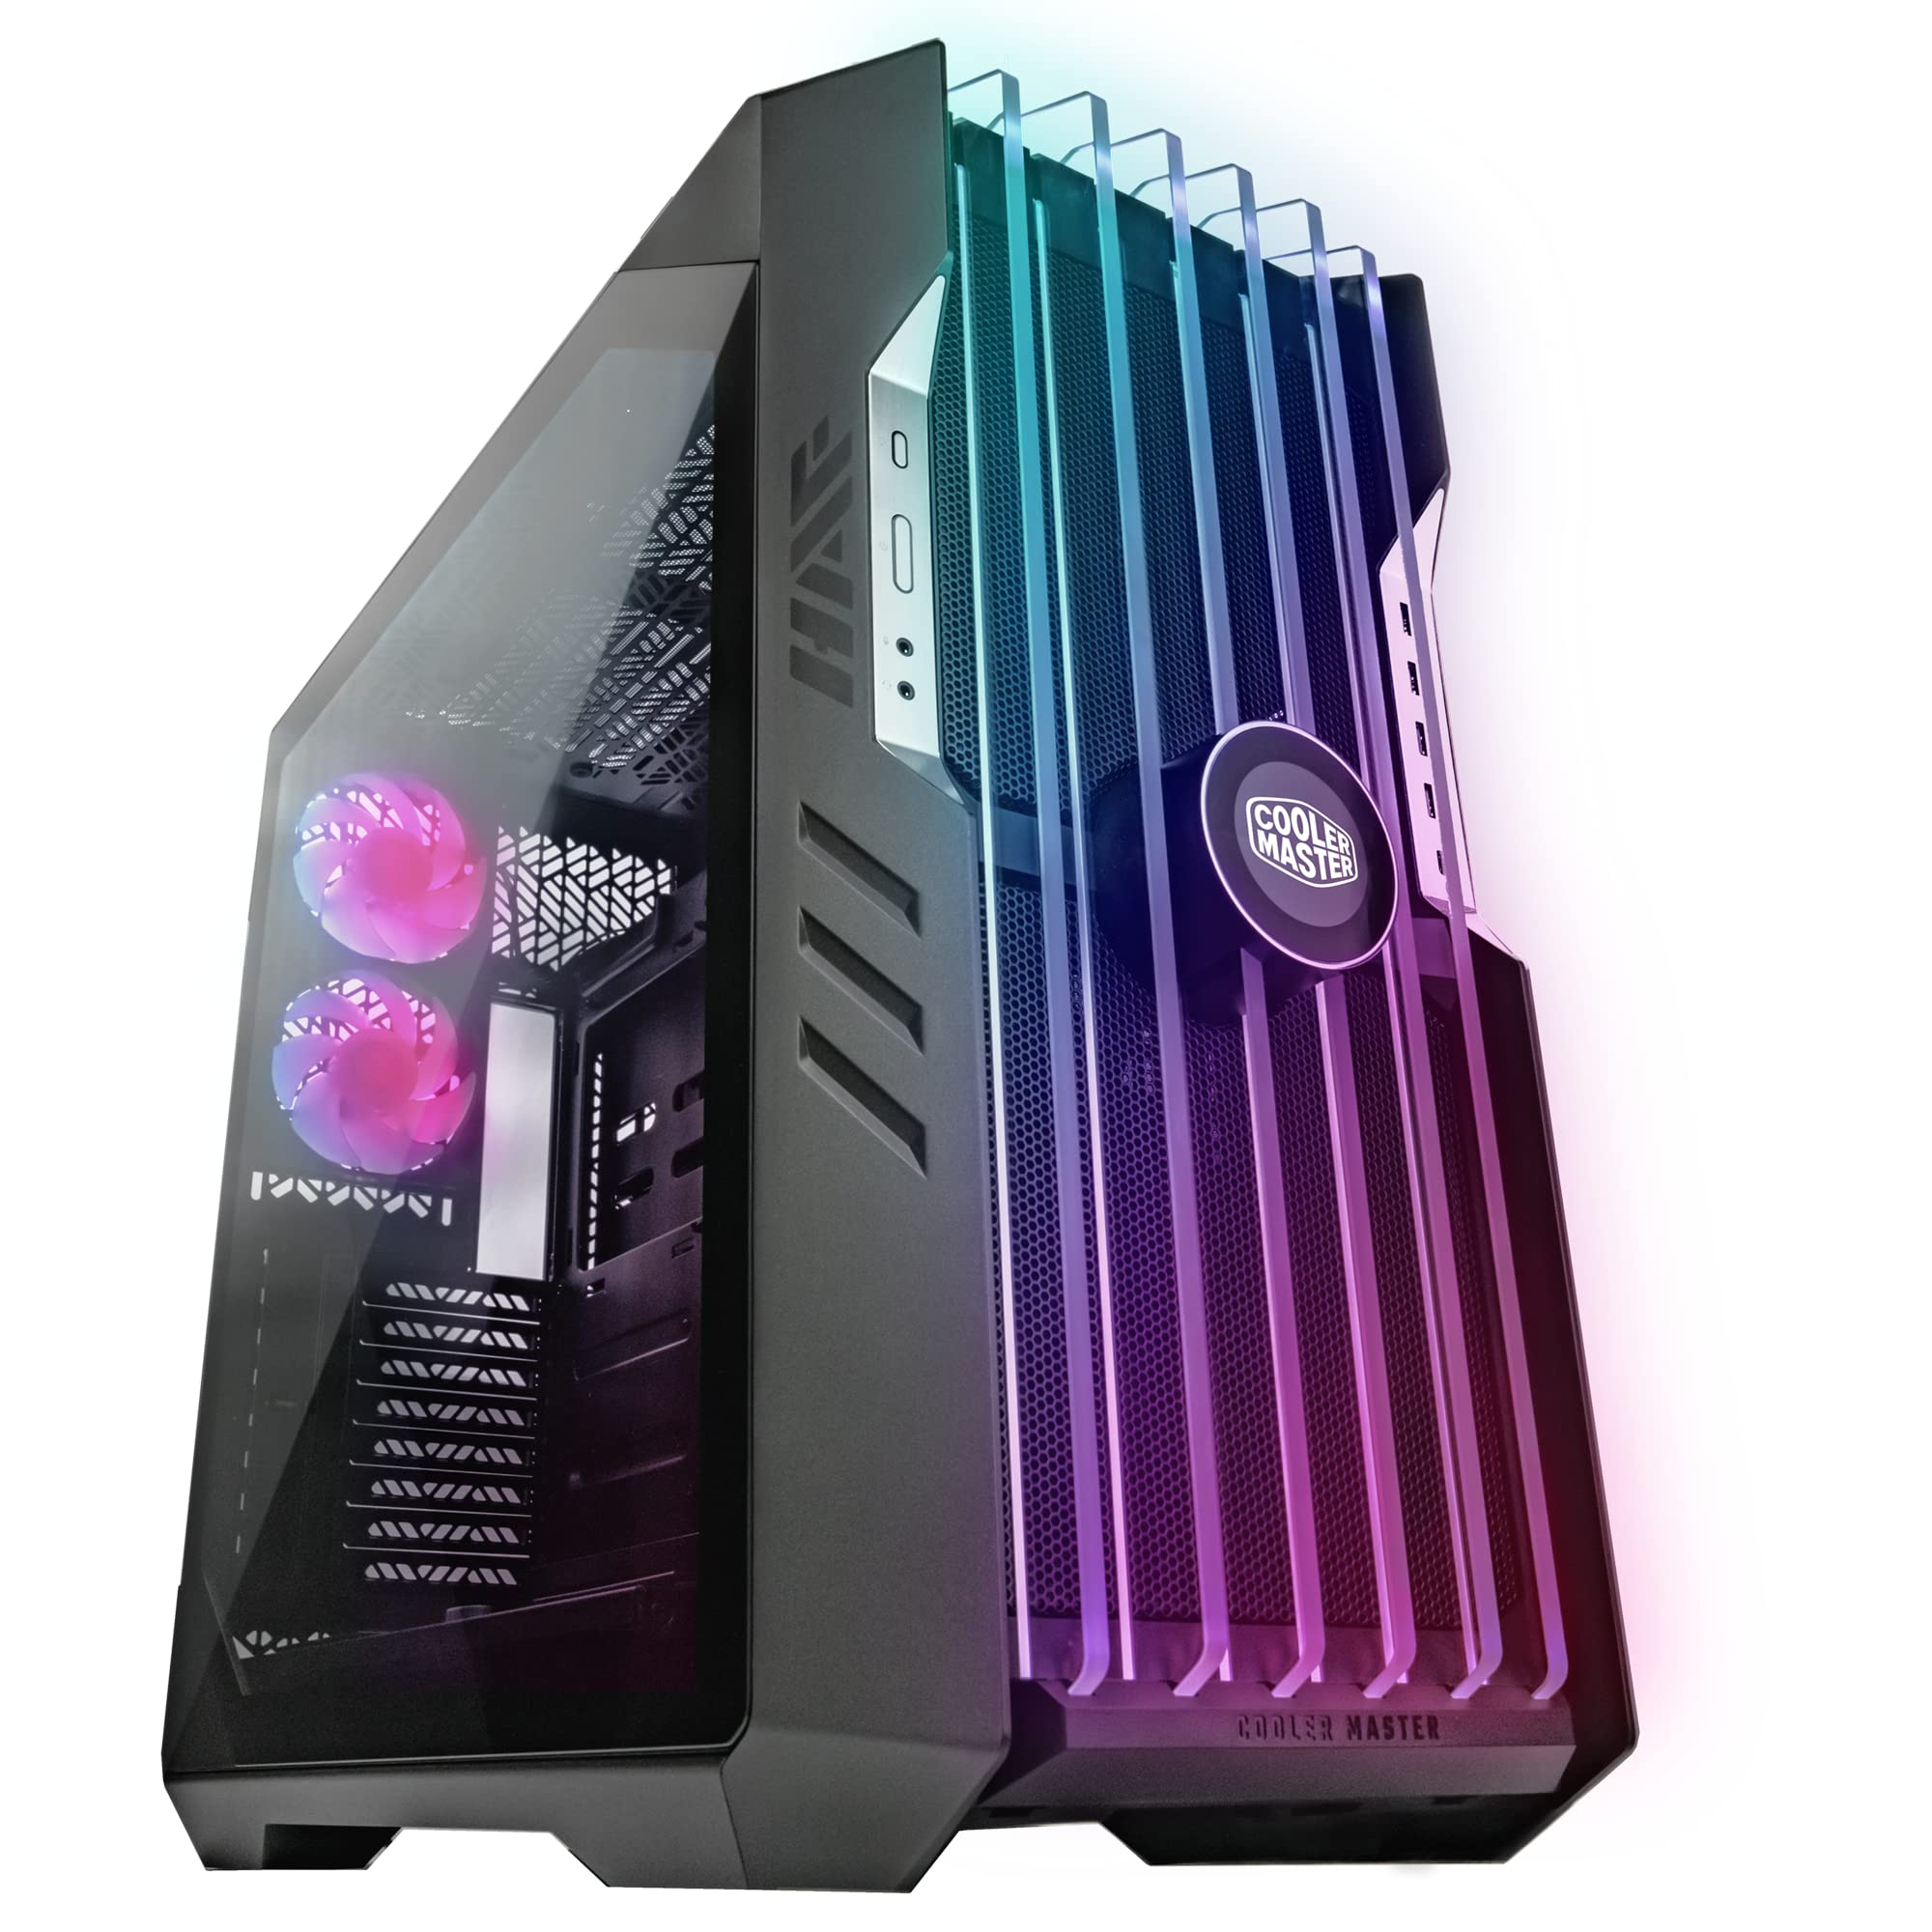
\includegraphics[scale=0.1]{Slike/kuciste.jpg}
    \caption{Cooler Master HAF 700 EVO}
    \label{fig:kuciste}
\end{figure}
Boja: titanium siva\\Dimenzije: 556 x 279 x 540 mm\\Podržani tipovi matičnih ploča: Mini ITX, Micro ATX, ATX, E-ATX, SSI CEB, SSI EEB\\\\Razlog: Oku ugodno kućište za RGB osvjetljenjem i izvrsnim protokom zraka radi optimalnih temperatura komponenti.\\\\  Cijena: 496,80 € - https://www.racunala.hr/cooler-master-haf700-evo-big-tower-schwarz-h700e-ignn-s00/224845/product/?utm\_source=nabava.net\&utm\_campaign=nabava.net\&utm\_medium=click

\pagebreak

\section{Napajanje: Corsair RM1000e}
\begin{figure}[H]
    \centering
    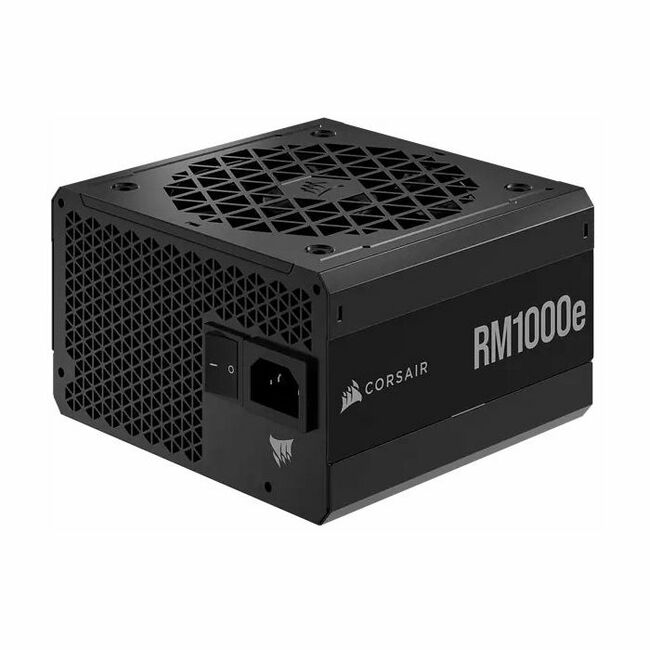
\includegraphics[scale=0.3]{Slike/napajanje.jpeg}
    \caption{Corsair RM1000e}
    \label{fig:enter-napajanje}
\end{figure}
ATX kabel: 1\\Snaga: 1000W\\Dimenzije: 140x150x86 mm\\MTBF: 100,000 sati\\Težina: 3,053kg\\Modularno: da\\\\Razlog: Kvalitetno napajanje s dovoljnom snagom od 1000W koje će biti potrebno za napajanje komponenti, također napajanje je modularno što će pridonijeti estetici rasporeda kabela po kućištu\\\\Cijena: 189,00 € - https://www.mikronis.hr/Proizvod/napajanje-corsair-rme-series-rm1000e-1000w-80-gold-fully-modular-atx-cp-9020264-eu/39577?utm\_source=nabava.net\&utm\_campaign=nabava.net\\\&utm\_medium=click

\pagebreak

\section{Hladnjak - CoolerMaster MasterLiquid PL360 FLUX}
\begin{figure}[H]
    \centering
    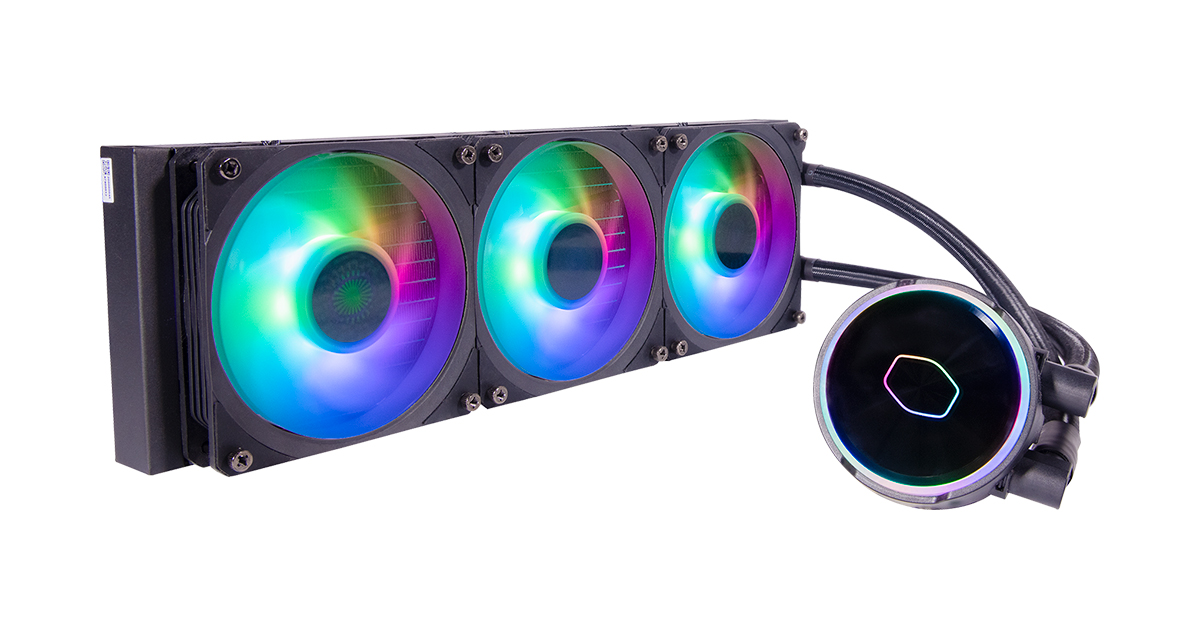
\includegraphics[scale=0.22]{Slike/hladnjak.jpg}
    \caption{CoolerMaster MasterLiquid PL360 FLUX}
    \label{fig:hladnjak}
\end{figure}
Podržani CPU Socket-i: LGA1700, LGA1200, LGA2066, LGA2011-v3, LGA2011, LGA1151, LGA1150, LGA1155, LGA1156, AM5, AM4, AM3+, AM3, AM2+, AM2, FM2+, FM2, FM1, TR4\\Materijal radijatora: aluminij\\Dimezije radijatora:394 x 119.6 x 27.2 mm \\Dimenzije pumpe:89 x 75 x 40 mm\\\\Razlog: Hladnjak koji ima potrebne specifikacije za hlađenje našeg procesora i održavanje istoga na niskim temperaturama.\\\\Cijena: 225,90 € - https://www.racunala.hr/cooler-master-pl360-flux-komplett-wasserkuhlung-schwarz-mly-d36m-a23pz-r1/228471/product/?utm\_source=nabava.net\&utm\_campaign=\\nabava.net\&utm\_medium=click

\pagebreak

\chapter{Periferija}

\section{Monitor - ROG Swift 360Hz PG27AQN}
\begin{figure}[H]
    \centering
    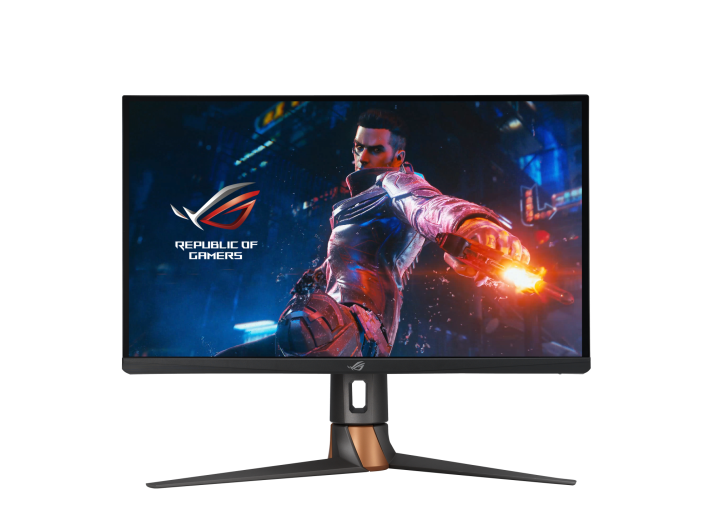
\includegraphics[scale=0.5]{monitor.png}
    \caption{ROG Swift 360Hz PG27AQN}
    \label{fig:monitor}
\end{figure}
Veličina: 27 inča\\Aspect ratio: 16:9\\Tip panela: fast IPS\\Rezolucija: 2560x1440\\Brzina osvježavanja: 360HZ\\\\Razlog: Odličan monitor precizno namijenjen igranju videoigara, visoka brzina osvježavanja i 1440p rezolucija doprinjet će uživanju u videoigrama.\\\\Cijena: 1.455,89 € - https://www.instar-informatika.hr/monitor-asus-27-rog-swift-pg27aqn-fast-ips-gaming-nvidia-g-sync-36/224248/product/?utm\_source=nabava.net\&utm\_campaign=nabava.net\&utm\_medium=click

\pagebreak

\section{Miš - Logitech G PRO X Superlight}
\begin{figure}[H]
    \centering
    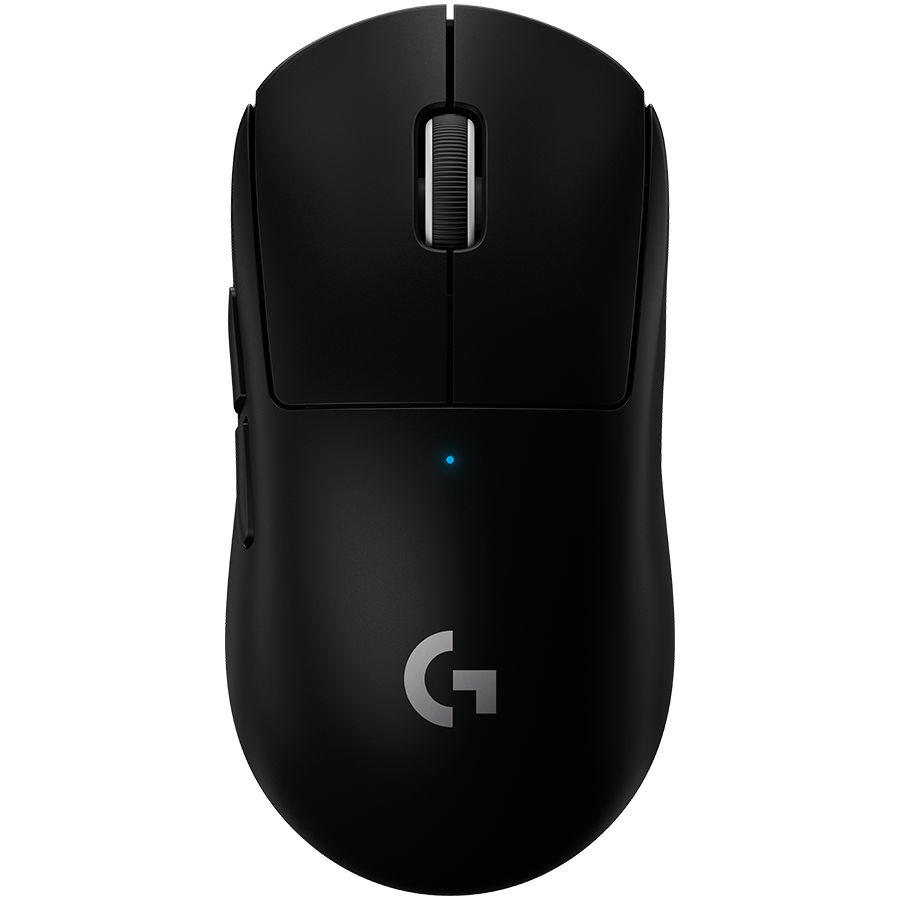
\includegraphics[scale=0.23]{miš.png}
    \caption{Logitech G PRO X Superlight}
    \label{fig:mis}
\end{figure}
Senzor: HERO\\DPI: 100 – 25,600 dpi\\Pooling rate: 1000Hz\\Baterija: 70 sati\\Težina: 63g\\\\Razlog: Ovaj miš koriste profesionalci diljem svijeta, preferiraju ga zbog odličnog dizajna koji savršeno prianja uz dlan i veoma niske težine od samo 63 grama.\\\\Cijena: 159,99 € - https://www.links.hr/hr/mis-logitech-pro-x-superlight-bezicni-opticki-25600dpi-bijeli-usb-101500580

\pagebreak

\section{Tipkovnica - HyperX Alloy Origins}
\begin{figure}[H]
    \centering
    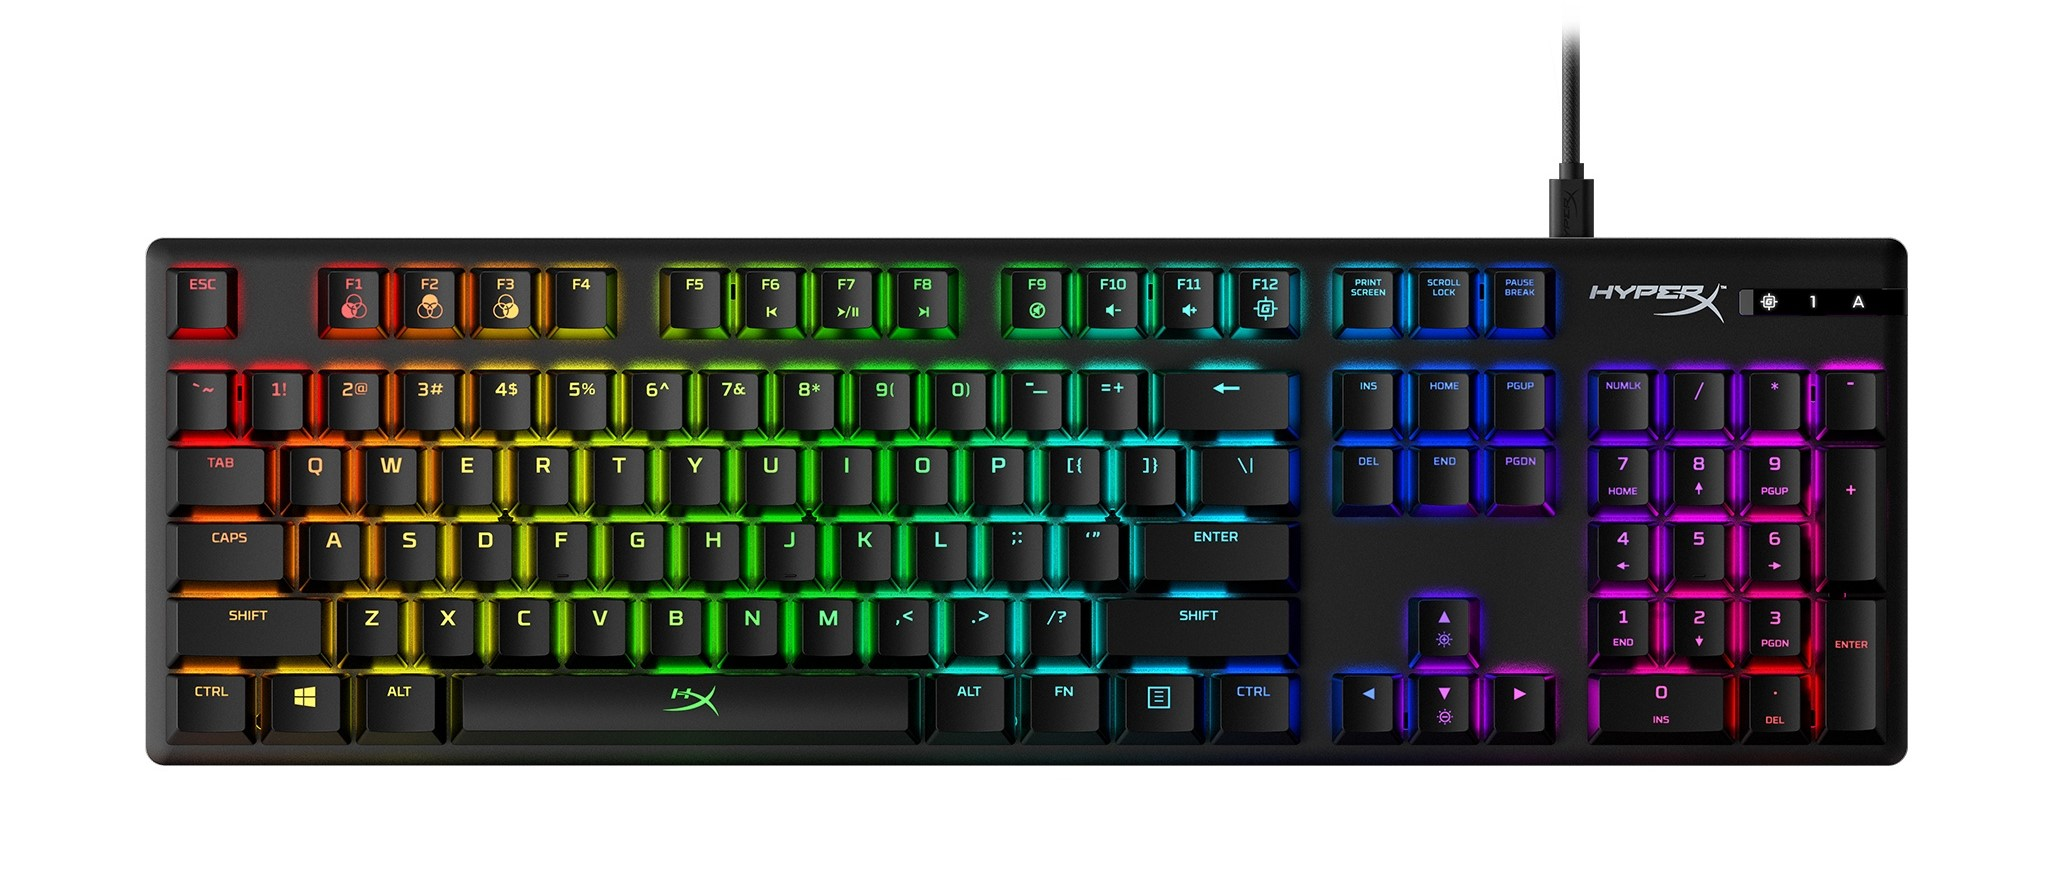
\includegraphics[scale=0.25]{Slike/tipkovnica.jpg}
    \caption{HyperX Alloy Origins}
    \label{fig:tipkovnica}
\end{figure}
Vrsta prekidača: Crveni\\Tip tipkovnice: Mehanička\\Osvjetljenje: RGB\\Težina: 1.1kg\\Raspored tipaka: US\\\\Razlog: Visokokvalitetna tipkovnica s crvenim prekidačima koji su namijenjeni za brzi odziv u videoigrama.\\\\Cijena: 139,99 € - https://www.links.hr/hr/tipkovnica-hyperx-alloy-origins-mehanicka-hyperx-red-crna-hx-kb6rdx-us-usb-101200508

\pagebreak

\chapter{Ukupna cijena računala}
Cijena komponenti: 5432,03 €\\Cijena periferije: 1755,87 €\\------------------------------------------\\Ukupna cijena: 7187,9 €

\end{document}
